\documentclass[a4j,titlepage]{jarticle}
\usepackage[dvipdfmx]{graphicx}
\usepackage{ascmac}
\usepackage{float}
\usepackage{amssymb}%にやりイコールを使う
\usepackage{multirow}
\usepackage{multicol}
\usepackage{tabularx}
%\usepackage{color}

\begin{document}

\title{2022 年度 3 回生前期学生実験 HW  \\ \bf team02 機能設計仕様書 植田健斗担当分}
% ↓ここに自分の氏名を記入
\author{機能設計仕様書作成者:植田健斗\\
グループメンバー:\\伊藤舜一郎 (学籍番号:1029-32-7548)
\\植田健斗 (学籍番号:1029-32-6498)}
\西暦
\date{提出期限:5月12日18時 提出日: \today} % コンパイル時の日付が自動で挿入される
\maketitle
\newpage


\section{全体のコンポーネント分割方法}

%\subsection{設計する回路の仕様}
%\subsection{設計の詳細}
%\subsubsection{ピン割当て}
%\subsection{正しく動作したか}
それぞれの機能を持った回路ごとにモジュール分割した。
各回路につけたファイル名は図\ref{moduleSplit0422}に示した通りである。(次の章の図\ref{rolesDivision0422}でまとめてある。)


\begin{figure}[H]
    \begin{center}
    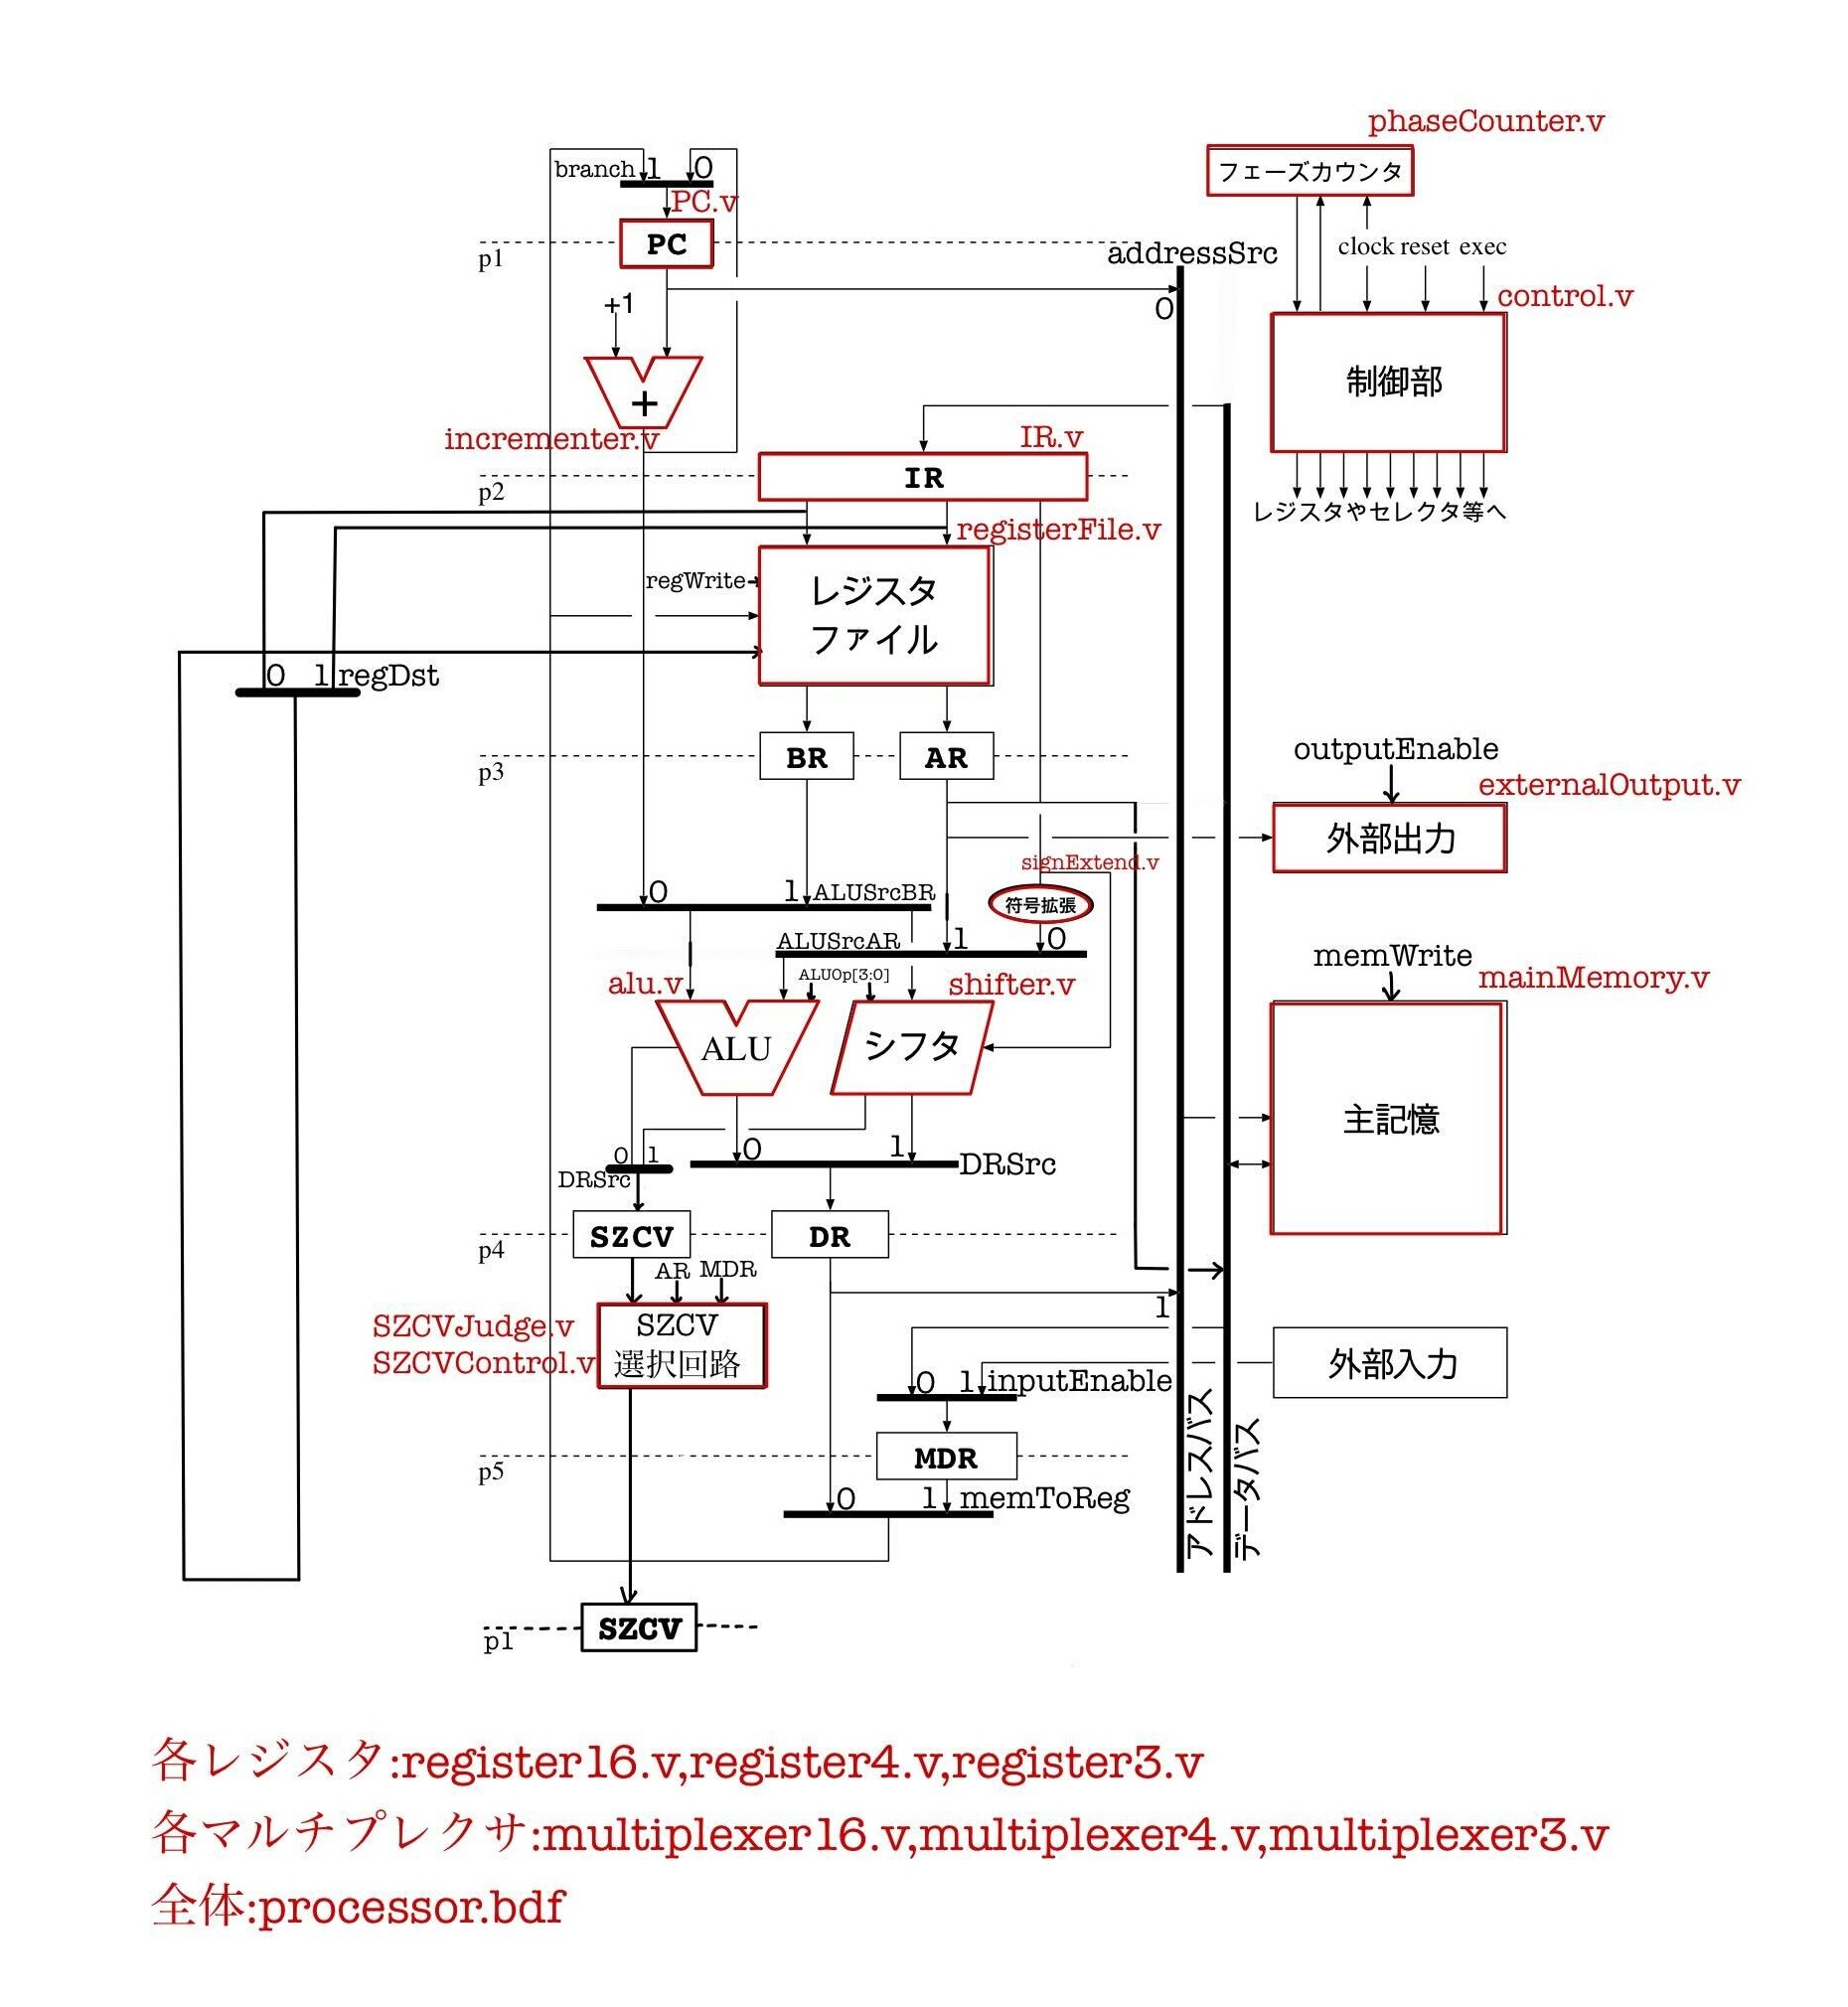
\includegraphics[scale = 0.22]{structure0506.jpg}
    \end{center}
    \caption{コンポーネント分割の方法の図}
    \label{moduleSplit0422}
\end{figure}

役割分担の表を以下の図\ref{rolesDivision0422}に示す。

\begin{figure}[H]
    \begin{center}
        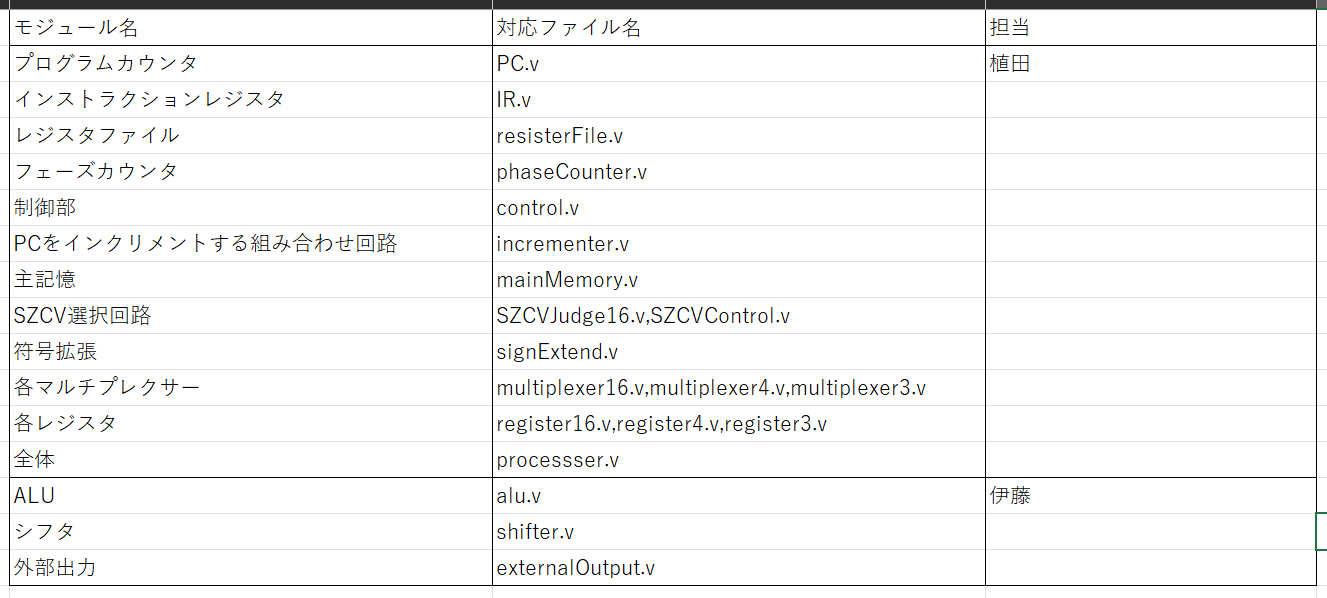
\includegraphics[scale = 0.42]{rolesDivision0506.png}
    \end{center}
    \caption{役割分担(4月22日時点)}
    \label{rolesDivision0422}
\end{figure}


\section{設計を担当したコンポーネント}
設計を担当したコンポーネントは以下である。
\begin{itemize}
    \item プログラムカウンタ(PC.v)
    \item インストラクションレジスタ(IR.v)
    \item レジスタファイル(registerFile.v)
    \item フェーズカウンタ(phaseCounter.v)
    \item 制御部(control.v)
    \item PCをインクリメントする組み合わせ回路(incrementer.v)
    \item 主記憶(mainMemory.v)
    \item SZCV選択回路(SZCVJudge16.v,SZCVControl.v)
    \item 符号拡張(signExtend.v)
    \item 各マルチプレクサー(multiplexer16.v,multiplexer4.v,multiplexer3.v)
    \item イネーブル・レジスタ(register16.v,register4.v,register3.v)
    \item 全体(processor.bdf)
\end{itemize}
各コンポーネントごとに外部仕様と内部仕様の説明を行う。




\newpage
\subsection{プログラムカウンタ(PC.v)}

\subsubsection{外部仕様 入力}
この回路の入力は以下の表\ref{ProgramCounterI}のようになる。
\begin{table}[H]
    \caption{プログラムカウンタ(PC.v)の入力(=input)}
    \label{ProgramCounterI}
    \begin{center}
    \begin {tabularx}{150mm}{|c|X|} \hline
         input & inputの説明 \\ \hline \hline
	 d[15:0] & クロックの立ち上がりにレジスタ書き込み可能ならば、内部のレジスタに書きこむ値\\ \hline
     clock & クロック信号。clockの立ち上がりで、レジスタ書きこみが可能な場合、書きこみが行われる。\\ \hline %%%%%
     changeEnable & 内部のレジスタが書き換え可能かを表す信号(イネーブル信号)。この信号が1のときにclockが立ち上がると内部のレジスタの値が更新される。 \\ \hline
     reset & 初期化信号。resetが1のときにクロックが立ち上がると、レジスタの中身を0で初期化する。\\ \hline
    \end{tabularx}
    \end{center}
\end{table}

\subsubsection{外部仕様 出力}
この回路の出力は以下の表\ref{ProgramCounterO}のようになる。
\begin{table}[H]
    \caption{プログラムカウンタ(PC.v)の出力(=output)}
    \label{ProgramCounterO}
    \begin{center}
    \begin {tabularx}{150mm}{|c|X|} \hline
     output & outputの説明 \\ \hline \hline
	 q[15:0] & プログラムカウンタに格納されている値で、命令を読みだすアドレスである。\\ \hline %%%%%
\end {tabularx}
    \end{center}
\end{table}

\subsubsection{内部仕様}
モジュールregister16.vとおなじ仕様である。
resetのときに格納する値を
変えやすくして保守性を高めるために、
register16.vと分けてモジュール化した。

%%%%%%%%%%%%%%%%%%%%%%%%%%%

\newpage
\subsection{インストラクションレジスタ(IR.v)}

\subsubsection{外部仕様 入力}
この回路の入力は以下の表\ref{aaaI}のようになる。
\begin{table}[H]
    \caption{インストラクションレジスタ(IR.v)の入力(=input)}
    \label{aaaI}
    \begin{center}
    \begin {tabularx}{150mm}{|c|X|} \hline
         input & inputの説明 \\ \hline \hline
         d[15:0] & クロックの立ち上がりにレジスタ書き込み可能ならば、内部のレジスタに書きこむ値\\ \hline
         clock & クロック信号。clockの立ち上がりで、レジスタ書きこみが可能な場合、書きこみが行われる。\\ \hline %%%%%
         changeEnable & 内部のレジスタが書き換え可能かを表す信号(イネーブル信号)。この信号が1のときにclockが立ち上がると内部のレジスタの値が更新される。\\ \hline
         reset & 初期化信号。resetが1のときにクロックが立ち上がると、レジスタの中身を16'b 1100000011100000で初期化する。\\ \hline
    \end{tabularx}
    \end{center}
\end{table}

\subsubsection{外部仕様 出力}
この回路の出力は以下の表\ref{aaaO}のようになる。
\begin{table}[H]
    \caption{インストラクションレジスタ(IR.v)の出力(=output)}
    \label{aaaO}
    \begin{center}
    \begin {tabularx}{150mm}{|c|X|} \hline
         output & outputの説明 \\ \hline \hline
         q[15:0] & IRに格納されている値で、主記憶から読みだされた命令である。\\ \hline
    \end {tabularx}
    \end{center}
\end{table}

\subsubsection{内部仕様}
モジュールregister16.vとほとんどおなじ仕様である。
resetのときに格納する値を16'b 1100000011100000(NOP命令を表す命令列)にしている点が異なる。


%%%%%%%%%%%%%%%%%%%%%%%%%%%


\newpage
\subsection{レジスタファイル(registerFile.v)}

\subsubsection{外部仕様 入力}
この回路の入力は以下の表\ref{registerFileI}のようになる。
\begin{table}[H]
    \caption{レジスタファイル(registerFile.v)の入力(=input)}
    \label{registerFileI}
    \begin{center}
    \begin {tabularx}{150mm}{|c|X|} \hline
         input & inputの説明 \\ \hline \hline
         Rs[2:0] & 命令中のRs・Raフィールドを受け取る。\\ \hline
         Rd[2:0] & 命令中のRd・Rbフィールドを受け取る。\\ \hline
         regWrite & 内部のレジスタが書き換え可能かを表す信号 regWriteとchangeEnableがともに1のときのみ書き換え可能\\ \hline
         writeData[15:0] & レジスタに書き込むデータ\\ \hline
         writeRegister[2:0] & writeData[15:0]を書きこむレジスタの番号\\ \hline
         clock & クロック信号。clockの立ち上がりで、レジスタ書きこみが可能な場合、書きこみが行われる。\\ \hline
         reset & 初期化信号。resetが1のときにクロックが立ち上がると、レジスタの中身を0で初期化する。\\ \hline
         changeEnable & 内部のレジスタが書き換え可能かを表す信号。regWriteとchangeEnableがともに1のときのみ書き換え可能\\ \hline
    \end{tabularx}
    \end{center}
\end{table}

\subsubsection{外部仕様 出力}
この回路の出力は以下の表\ref{registerFileO}のようになる。
\begin{table}[H]
    \caption{レジスタファイル(registerFile.v)の出力(=output)}
    \label{registerFileO}
    \begin{center}
    \begin {tabularx}{150mm}{|c|X|} \hline
         output & outputの説明 \\ \hline \hline
         AR[15:0] & Rs(Ra)フィールドで指定したレジスタに格納されているデータを読み込む。 \\ \hline
         BR[15:0] & Rd(Rb)フィールドで指定したレジスタに格納されているデータを読み込む。 \\ \hline
    \end {tabularx}
    \end{center}
\end{table}

\subsubsection{内部仕様}
内部に8個の16bitレジスタreg [15:0] r [7:0]を持ち、
入力Rs[2:0],Rd[2:0]の値に応じたレジスタに格納されたデータを
それぞれAR[15:0],BR[15:0]として出力する。
また、resetが0でchangeEnableとregWriteがともに1のときのみ書き換え可能状態になり、
この状態でclockが立ち上がると、入力writeData[15:0]で受け取ったデータを
writeRegister[2:0]に対応する番号の内部レジスタrにデータを書きこむ。

resetが1のときにclockが立ち上がると、
すべての内部レジスタrの値を0で初期化する。

このレジスタファイルはパイプライン化をするにあたって改良の余地がある。
あるレジスタへの書き込みとそのレジスタからのデータの読み出しを
同じクロック周期の中で行ったときに、
中間報告時点で作成したレジスタファイルでは、
書き込みを行う前のデータが読みだされてしまう。
最終課題までには、
あるレジスタへの書き込みとそのレジスタからのデータの読み出しを
同じクロック周期の中で行ったときに、
同じクロックの中で書き込みするデータを読みだせるように
改良をする必要がある。



%%%%%%%%%%%%%%%%%%%%%%%%%%%


\newpage
\subsection{フェーズカウンタ(phaseCounter.v)}

\subsubsection{外部仕様 入力}
この回路の入力は以下の表\ref{phaseCounterI}のようになる。
\begin{table}[H]
    \caption{フェーズカウンタ(phaseCounter.v)の入力(=input)}
    \label{phaseCounterI}
    \begin{center}
    \begin {tabularx}{150mm}{|c|X|} \hline
         input & inputの説明 \\ \hline \hline
         clock & クロック信号。clock立ち上がりで、レジスタ書きこみが可能な場合、書きこみが行われる。 \\ \hline
         reset & 初期化信号。resetが1のときにクロックが立ち上がると、フェーズをp1に戻す。\\ \hline 
         changeEnable & 内部のレジスタが書き換え可能かを表す信号(イネーブル信号)。この信号が1のときにclockが立ち上がると内部のレジスタの値が更新される。\\ \hline
    \end{tabularx}
    \end{center}
\end{table}

\subsubsection{外部仕様 出力}
この回路の出力は以下の表\ref{phaseCounterO}のようになる。
\begin{table}[H]
    \caption{フェーズカウンタ(phaseCounter.v)の出力(=output)}
    \label{phaseCounterO}
    \begin{center}
    \begin {tabularx}{150mm}{|c|X|} \hline
         output & outputの説明 \\ \hline \hline
         p1 & p1フェーズを表す信号。IRのイネーブル信号に使われる。\\ \hline
         p2 & p2フェーズを表す信号。AR,BRのイネーブル信号に使われる。\\ \hline %%%%%
         p3 & p3フェーズを表す信号。外部出力、SZCV,DRのイネーブル信号に使われる。\\ \hline
         p3to4 & p3とp4の間で立ち上がる信号。メモリのイネーブル信号に使われる。\\ \hline
         p4 & p4フェーズを表す信号。MDRのイネーブル信号に使われる。\\ \hline
         p5 & p5フェーズを表す信号。SZCV選択回路を通過した後のSZCV,レジスタファイル,PCのイネーブル信号に使われる。\\ \hline
    \end {tabularx}
    \end{center}
\end{table}

\subsubsection{内部仕様}
クロックの立ち上がりごとに
p1$\rightarrow$p2$\rightarrow$p3$\rightarrow$p4$\rightarrow$p5の順に
フェーズ信号が立ち上がる。
マスタースレーブ方式のdffを用いてクロックの立ち上がりから
半周期ずらしてp1からp5のフェーズ信号が立ち上がるようにしている。
またp3とp4の間にp3to4という信号が立ち上がる。
各信号の時間変化は以下の図\ref{phaseCounterWaveShape}のようになる。
クロックの立下りのタイミングでp1からp5の各フェーズ信号が立ち上がっていて、
p3top4だけclockの立ち上がりのタイミングにに立ち上がっている。
各フェーズ信号は5クロックごとに立ち上がっている。

\begin{figure}[H]
    \begin{center}
        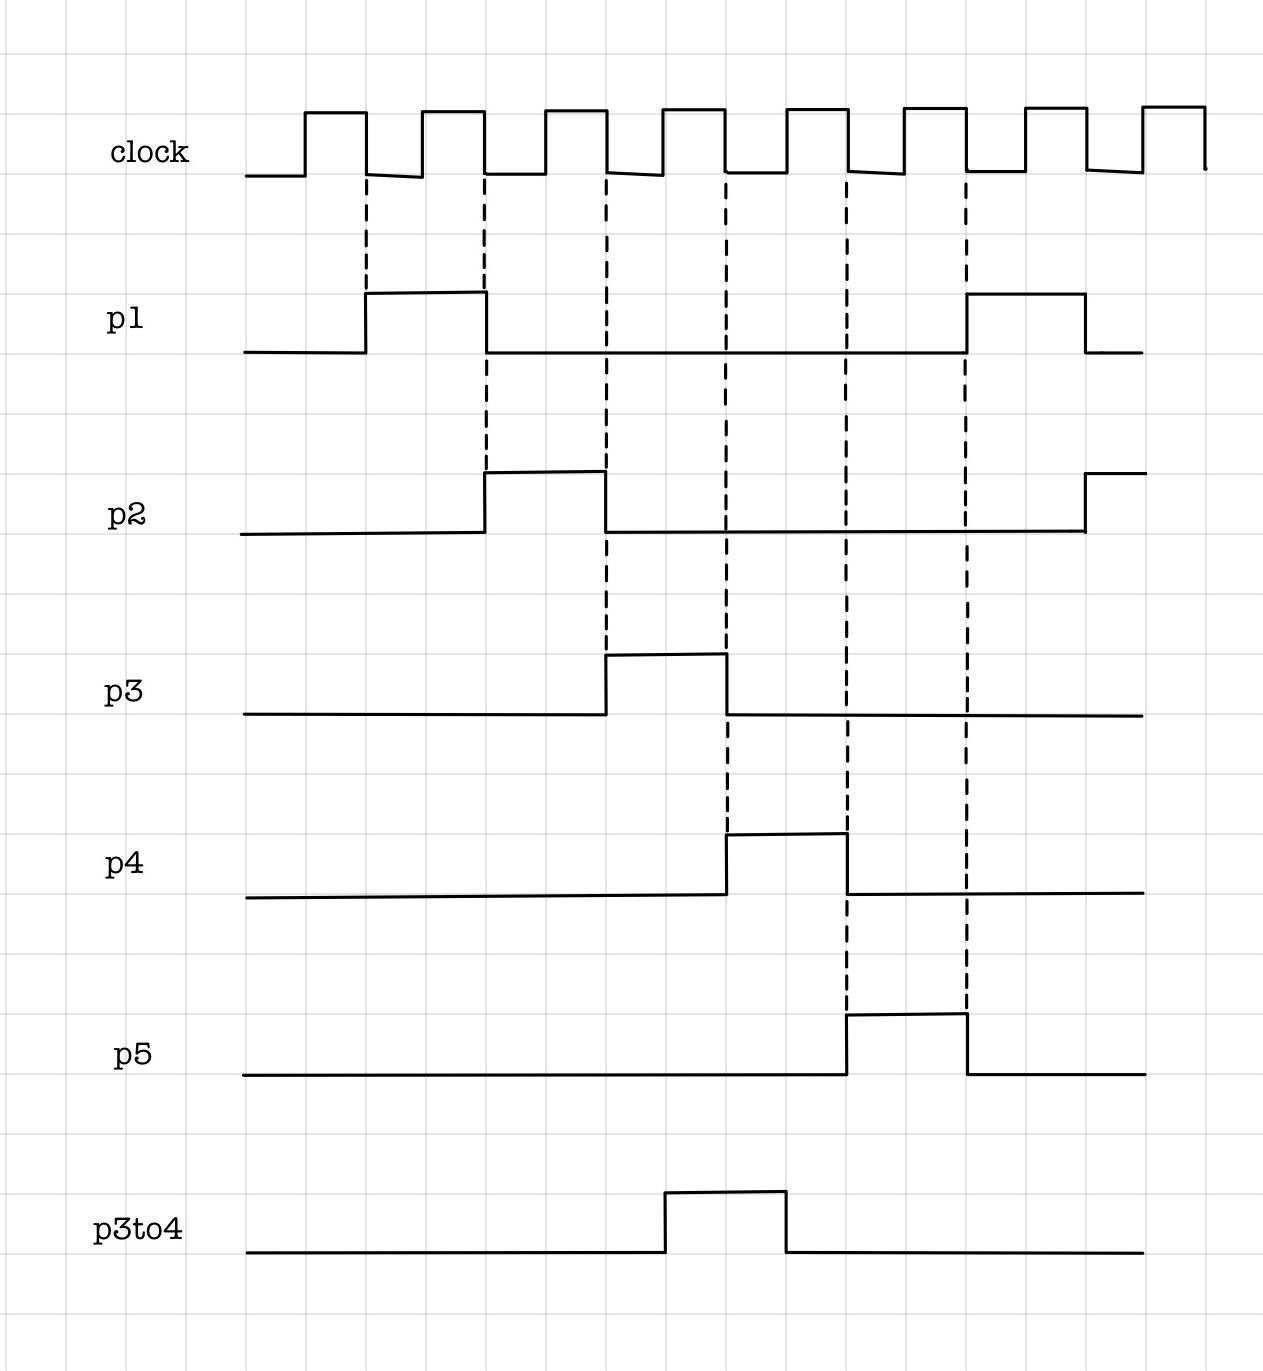
\includegraphics[scale = 0.22]{phaseCounterWaveShape.jpg}
    \end{center}
    \caption{フェーズカウンタの各信号の時間変化}
    \label{phaseCounterWaveShape}
\end{figure}


%%%%%%%%%%%%%%%%%%%%%%%%%%%


\newpage
\subsection{制御部(control.v)}

\subsubsection{外部仕様 入力}
この回路の入力は以下の表\ref{controlI}のようになる。
\begin{table}[H]
    \caption{制御部(control.v)の入力(=input)}
    \label{controlI}
    \begin{center}
    \begin {tabularx}{150mm}{|c|X|} \hline
         input & inputの説明 \\ \hline \hline
         clock & クロック信号。clock立ち上がりで、レジスタ書きこみが可能な場合、書きこみが行われる。 \\ \hline 
         instruction[15:0] & 命令の格納されたIRの出力を受け取る。 \\ \hline 
         reset & 初期化信号。resetが1のときにクロックが立ち上がると、出力systemRunning信号を0にする。 \\ \hline
         exec & 全体の実行・停止信号execを受け取る。\\ \hline
         p1 & フェーズカウンタの出力p1を受け取る。\\ \hline
         p2 & フェーズカウンタの出力p2を受け取る。\\ \hline
         p3 & フェーズカウンタの出力p3を受け取る。\\ \hline
         p3to4 & フェーズカウンタの出力p3to4を受け取る。\\ \hline
         p4 & フェーズカウンタの出力p4を受け取る。\\ \hline
         p5 & フェーズカウンタの出力p5を受け取る。\\ \hline
         SZCV[3:0] & 前回の命令でのSZCVフラグを受け取る。\\ \hline
    \end{tabularx}
    \end{center}
\end{table}

\subsubsection{外部仕様 出力}
この回路の出力は以下の表\ref{controlO}のようになる。
\begin{table}[H]
    \caption{制御部(control.v)の出力(=output)}
    \label{controlO}
    \begin{center}
    \begin {tabularx}{150mm}{|c|X|} \hline
         output & outputの説明 \\ \hline \hline
         addressSrc & メモリに入力するアドレスが、IRの値(=0)かDRの値(=1)かを決める。\\ \hline
         regDst & 書き込みをするレジスタを、入力Instruction[10:8](Rd,Rbフィールド)で指定する(=0)か、Instruction[13:11](Ra,Rsフィールド)で指定する(=1)かを決める。\\ \hline %%%%%
         ALUSrcAR & ALUの入力inB[15:0]の受け取る値が、命令中の即値(=0)か、ARの値(=1)かを決める。\\ \hline
         ALUSrcBR & ALUの入力inA[15:0]の受け取る値が、((プログラムカウンタの値)+1)にする(=0)かBRの値にするか(=1)かを決める。\\ \hline
         ALUOp[3:0] & ALUの入力op[3:0]に入力する値で、ALUで行う演算を決める。\\ \hline
         DRSrc & DRに入力する値を、ALUの出力out[15:0]にする(=0)か、シフタの出力out[15:0]にする(=1)かを決める。
         また、SZCVに入力する値を、ALUの出力SZCV[3:0]にする(=0)か、シフタの出力SZCV[3:0]にする(=1)かを決める。\\ \hline
         outputEnable & 外部出力に値を受け渡す(=1)か受け渡さない(=0)かを決める。正確にはOUT命令のときのみ1となる。\\ \hline
         inputEnable & 外部入力から値を受け取る(=1)か受け取らない(=0)かを決める。正確にはIN命令のときのみ1となる。\\ \hline
         memWrite & メモリに書きこむ(=1)か書きこまない(=0)かを決める。正確にはST命令のときのみ1となる。\\ \hline
         branch & 入力のSZCV[3:0]とinstruction[15:0]から、分岐をする(=1)か、分岐をしない(=0)かを決める。\\ \hline
         regWrite & レジスタファイルに書き込みを行う(=1)か、レジスタファイルに書き込みを行わない(=0)かを決める。\\ \hline
         memToReg & プログラムカウンタや、レジスタファイルに渡すデータを、DRの値にする(=0)かMDRの値にする(=1)かを決める。\\ \hline
         systemRunning & すべてのレジスタの書き換えを不可能にする(=0)か可能にする(=1)かを決める。
         つまり、機械が実行待機状態(=0)か動作状態(=1)かを決める。\\ \hline
    \end {tabularx}
    \end{center}
\end{table}

\subsubsection{内部仕様}
systemRunningという1bitの内部レジスタを持ち、
その値を変えることで機械を実行待機状態(systemRunning=0)か実行状態(systemRunning=1)かを
切り替えている。
exec入力については1クロック前のexec入力を保持する1bitレジスタexec\_preと
カウンタを表す16bitの内部レジスタcounterを
持つ。これを用いて以下の表\ref{execexecprecntsystemRunningRelation}のようにexecとexec\_preの値に応じて、
counterとsystemRunningを変更する。これによりexecボタンのチャタリングを除去しながら、
execボタンが押されるたびに
機器が実行状態かどうかを決めるsystemRunningを反転させることができる。


\begin{table}[H]
    \caption{execとexec\_preとcnt(=counter)の値に応じて、更新するcnt(=counter)とsystemRunningの値}
    \label{execexecprecntsystemRunningRelation}
    \begin{center}
    \begin {tabularx}{145mm}{|c||cccX|} \hline
         exec\_pre exec & 00 & 01 & 10 & 11 \\ \hline \hline
         cnt=0 & cnt\textless =0 & cnt\textless =1 & cnt\textless =1 & cnt\textless =0 \\ \hline
         0\textless cnt\textless 15 & cnt\textless =cnt+1 & cnt\textless =0 & cnt\textless =0 & cnt\textless =cnt+1 \\ \hline
         cnt=15 & cnt\textless =0 & cnt\textless =0 & cnt\textless =0 & cnt\textless =0,              sysstemRunning\textless =$\sim$sysstemRunning \\ \hline 

    \end {tabularx}
    \end{center}
\end{table}

resetが呼ばれると、
\begin{verbatim} 
    counter <= 16'h 0000;
    systemRunning <= 1'b 0;
    exec_pre <= exec;
\end{verbatim}
により初期化を行う。
resetが押されるとsystemRunningは0になるので、
実行が停止し、実行待機状態になる。その後execボタンが押されることで
systemRunningが1になり実行が行われるようになる。
また、インプット命令のp3と
halt命令のp5のフェーズでsystemRunningを0にし
実行待機状態になるようにしている。
この場合もexecボタンを押すことで実行を再開できる。


各制御信号は組み合わせ回路を用いて実現している。
以下の表\ref{controlsignal}でそれぞれの制御信号の出力の仕様をまとめた。


\begin{table}[H]
    \caption{制御信号の仕様}
    \label{controlsignal}
    \begin{center}
    \begin{tabularx}{150mm}{|c|X|} \hline
         制御信号名 & 制御信号の仕様  \\ \hline \hline
         addressSrc & =p3to4 \\ \hline
         regDst & LD命令の時のみ1 \\ \hline %%%%%
         ALUSrcAR & 演算,シフト,IN,OUT,NOP,HALT命令の時に1になる。(MOVの下のreservedの時も1) \\ \hline
         ALUSrcBR & 演算、シフト、IN,OUT,NOP,HALT,LD,ST命令の時に1になる。(MOVの下のreservedの時も1) \\ \hline
         ALUOp[3:0] & 演算命令(MOVの下のreservedも含む)のときはinstruction[7:4](命令で指定した演算)になる。LI命令の時は4'b 0110(MOV命令)になる。その他のときは4'b 0000(アドレス計算のための足し算)になる。 \\ \hline
         DRSrc & シフト,IN,OUT,NOP,HALT命令の時のみ1 \\ \hline
         outputEnable & OUT命令の時のみ1 \\ \hline
         inputEnable & IN命令の時のみ1 \\ \hline
         memWrite & ST命令の時のみ1 \\ \hline
         branch & B命令または(BE命令かつZ=1)または(BLT命令かつS\textasciicircum V=1)または(BLE命令かつZ\textbar (S\textasciicircum V)=1)または(BNEかつ$\sim$Z=1)のときのみ1 \\ \hline
         regWrite & ADD,SUB,AND,OR,XOR,MOV,シフト,IN,LD,LI命令の時のみ1 \\ \hline
         memToReg & LD,IN命令の時のみ1 \\ \hline
    \end{tabularx}
    \end{center}
\end{table}


%%%%%%%%%%%%%%%%%%%%%%%%%%%


\newpage
\subsection{PCをインクリメントする組み合わせ回路(incrementer.v)}

\subsubsection{外部仕様 入力}
この回路の入力は以下の表\ref{incrementerI}のようになる。
\begin{table}[H]
    \caption{PCをインクリメントする組み合わせ回路(incrementer.v)の入力(=input)}
    \label{incrementerI}
    \begin{center}
    \begin {tabularx}{150mm}{|c|X|} \hline
         input & inputの説明 \\ \hline \hline
         pc\_pre[15:0] & プログラムカウンタの値を受け取る。\\ \hline
    \end{tabularx}
    \end{center}
\end{table}

\subsubsection{外部仕様 出力}
この回路の出力は以下の表\ref{incrementerO}のようになる。
\begin{table}[H]
    \caption{PCをインクリメントする組み合わせ回路(incrementer.v)の出力(=output)}
    \label{incrementerO}
    \begin{center}
    \begin {tabularx}{150mm}{|c|X|} \hline
         output & outputの説明 \\ \hline \hline
         pc\_post[15:0] & pc\_post = pc\_pre + 1\\ \hline
    \end {tabularx}
    \end{center}
\end{table}

\subsubsection{内部仕様}
プログラムカウンタの値を受け取り加算器を用いてインクリメントした後出力する。
pc\_post = pc\_pre + 1を実行する。
%%%%%%%%%%%%%%%%%%%%%%%%%%%


\newpage
\subsection{主記憶(mainMemory.v)}

\subsubsection{外部仕様 入力}
この回路の入力は以下の表\ref{mainMemoryI}のようになる。
\begin{table}[H]
    \caption{主記憶(mainMemory.v)の入力(=input)}
    \label{mainMemoryI}
    \begin{center}
    \begin {tabularx}{150mm}{|c|X|} \hline
         input & inputの説明 \\ \hline \hline
         address[11:0] & メモリの読み書きを行う番地のアドレス。\\ \hline
         clock & クロック信号を反転させて入力する。clockの立ち上がり(=クロック信号の立ち下り)で、メモリ書きこみが可能な場合書きこみが行われ、また、
         address[11:0]により指定した番地のデータの読み出しが行われる。 \\ \hline 
         data[15:0] & メモリに書きこむためのデータ\\ \hline
         wren & 書き込み可能信号。この信号が1でかつclockが立ち上がった時にメモリに書き込みが行われる。\\ \hline
    \end{tabularx}
    \end{center}
\end{table}

\subsubsection{外部仕様 出力}
この回路の出力は以下の表\ref{mainMemoryO}のようになる。
\begin{table}[H]
    \caption{主記憶(mainMemory.v)の出力(=output)}
    \label{mainMemoryO}
    \begin{center}
    \begin {tabularx}{150mm}{|c|X|} \hline
         output & outputの説明 \\ \hline \hline
         q[15:0] & メモリから読み出しされたデータ\\ \hline
    \end {tabularx}
    \end{center}
\end{table}

\subsubsection{内部仕様}
RAMを用いて実装した。address[11:0]で指定した番地に対して、
clockが立ち上がる度にデータの読み出し・書き込みを行う。
書き込みはwren信号が1のときにしか行われない。

%%%%%%%%%%%%%%%%%%%%%%%%%%%


\newpage
\subsection{SZCV選択回路(SZCVJudge16.v)}

\subsubsection{外部仕様 入力}
この回路の入力は以下の表\ref{szcvjudgeI}のようになる。
\begin{table}[H]
    \caption{SZCV選択回路(SZCVJudge16.v)の入力(=input)}
    \label{szcvjudgeI}
    \begin{center}
    \begin {tabularx}{150mm}{|c|X|} \hline
         input & inputの説明 \\ \hline \hline
         data[15:0] & SZCVフラグを求めたいデータを受け取る。\\ \hline
    \end{tabularx}
    \end{center}
\end{table}

\subsubsection{外部仕様 出力}
この回路の出力は以下の表\ref{szcvjudgeO}のようになる。
\begin{table}[H]
    \caption{SZCV選択回路(SZCVJudge16.v)の出力(=output)}
    \label{szcvjudgeO}
    \begin{center}
    \begin {tabularx}{150mm}{|c|X|} \hline
         output & outputの説明 \\ \hline \hline
         SZCV[3:0] & 入力data[15:0]に応じたSZCVフラグを出力する。\\ \hline
    \end {tabularx}
    \end{center}
\end{table}

\subsubsection{内部仕様}
data[15:0]を符号付き16進数としたときにdata[15:0]が正ならSZCV[3:0]=4'b 0000,
data[15:0]が負ならSZCV[3:0]=4'b 1000,data[15:0]が0ならSZCV[3:0]=4'b 0100を出力する。
つまり、SZCV[3]=data[15],SZCV[2]=(data[15:0]==16'h 0000),SZCV[1]=0,SZCV[0]=0となっている。

%%%%%%%%%%%%%%%%%%%%%%%%%%%


\newpage
\subsection{SZCV選択回路(SZCVControl.v)}

\subsubsection{外部仕様 入力}
この回路の入力は以下の表\ref{szcvcontrolI}のようになる。
\begin{table}[H]
    \caption{SZCV選択回路(SZCVControl.v)の入力(=input)}
    \label{szcvcontrolI}
    \begin{center}
    \begin {tabularx}{150mm}{|c|X|} \hline
         input & inputの説明 \\ \hline \hline
         instruction[15:0] & 命令の格納されたIRの出力を受け取る。\\ \hline
    \end{tabularx}
    \end{center}
\end{table}

\subsubsection{外部仕様 出力}
この回路の出力は以下の表\ref{szcvcontrolO}のようになる。
\begin{table}[H]
    \caption{SZCV選択回路(SZCVControl.v)の出力(=output)}
    \label{szcvcontrolO}
    \begin{center}
    \begin {tabularx}{150mm}{|c|X|} \hline
         output & outputの説明 \\ \hline \hline
         SZCVSrc[1:0] & どのSZCVフラグを使うかを決める。
         ARのSZCVフラグを使う(=2'b 11)、
         ALU・シフタのSZCVフラグを使う(=2'b 00,2'b 10)、
         MDRのSZCVフラグを使う(=2'b 01)\\ \hline
    \end {tabularx}
    \end{center}
\end{table}

\subsubsection{内部仕様}
SZCVSrc[0]はIN,OUT,ST,LD命令の時に1になり、
SZCVSrc[1]はOUT,STのときに1になる
組み合わせ回路である。
これによりOUT,ST命令のときはARのSZCVフラグを、
IN,LD命令の時にはMDRのSZCVフラグを、
その他の命令のときにはALU・シフタで計算されたSZCVフラグを、
それぞれ選択できるようになっている。
SZCV選択回路自体はSZCVJudge.vとSZCVControl.vとmultiplexter4.vを用いて
、全体(processor.bdf)の中で構成している。
(つまり、SZCV選択回路自体の.vファイルは存在しない。)

(なぜこのようになっているかと言うとST命令のときのSZCVフラグの立て方を
授業資料で指定されていなかったので未定義にして設計をしたところ、フィボナッチ数列を
求めるテストケースではSTのSZCVフラグは格納するデータのSZCVフラグでなければ
いけないことになっていた。これにより急遽追加したのがSZCV選択回路である。この回路は
パイプライン処理で再利用ができないので不要になる。そのため、.vファイルを作ることをしなかった。
つまり、SZCV選択回路が当初の計画に組み込まれていなかったため、
この回路を全体(processor.bdf)の中で構成をすることになり、
全体の回路(processor.bdf)が見にくくなってしまったが、ご容赦ください。)
%%%%%%%%%%%%%%%%%%%%%%%%%%%


\newpage
\subsection{符号拡張(signExtend.v)}

\subsubsection{外部仕様 入力}
この回路の入力は以下の表\ref{signExtendI}のようになる。
\begin{table}[H]
    \caption{符号拡張(signExtend.v)の入力(=input)}
    \label{signExtendI}
    \begin{center}
    \begin {tabularx}{150mm}{|c|X|} \hline
         input & inputの説明 \\ \hline \hline
         in[7:0] & 符号拡張する8bitの数字を受け取る。 \\ \hline
    \end{tabularx}
    \end{center}
\end{table}

\subsubsection{外部仕様 出力}
この回路の出力は以下の表\ref{signExtendO}のようになる。
\begin{table}[H]
    \caption{符号拡張(signExtend.v)の出力(=output)}
    \label{signExtendO}
    \begin{center}
    \begin {tabularx}{150mm}{|c|X|} \hline
         output & outputの説明 \\ \hline \hline
         out[15:0] & 符号拡張後の16bitの数字を出力\\ \hline
    \end {tabularx}
    \end{center}
\end{table}

\subsubsection{内部仕様}

\begin{verbatim}
out[15:0] = {{8{in[7]}},in[7:0]}により、符号拡張を行う。
\end{verbatim}

%%%%%%%%%%%%%%%%%%%%%%%%%%%


\newpage
\subsection{各マルチプレクサー(multiplexer16.v,multiplexer4.v,multiplexer3.v)}

\subsubsection{外部仕様 入力}
この回路の入力は以下の表\ref{eachmultiplexerI}のようになる。
\begin{table}[H]
    \caption{各マルチプレクサー(multiplexer16.v,multiplexer4.v,multiplexer3.v)の入力(=input)}
    \label{eachmultiplexerI}
    \begin{center}
    \begin {tabularx}{150mm}{|c|X|} \hline
         input & inputの説明 \\ \hline \hline
         in0[15:0 or 3:0 or 2:0] & セレクタ信号が0の時に出力されるデータ\\ \hline
         in1[15:0 or 3:0 or 2:0] & セレクタ信号が1の時に出力されるデータ\\ \hline %%%%%
         selector & 1bitのセレクタ信号\\ \hline
    \end{tabularx}
    \end{center}
\end{table}

\subsubsection{外部仕様 出力}
この回路の出力は以下の表\ref{eachmultiplexerO}のようになる。
\begin{table}[H]
    \caption{各マルチプレクサー(multiplexer16.v,multiplexer4.v,multiplexer3.v)の出力(=output)}
    \label{eachmultiplexerO}
    \begin{center}
    \begin {tabularx}{150mm}{|c|X|} \hline
         output & outputの説明 \\ \hline \hline
         out[15:0] & in0またはin1のうち、セレクタ信号により選ばれた方のデータの値になる。\\ \hline
    \end {tabularx}
    \end{center}
\end{table}

\subsubsection{内部仕様}
\begin{verbatim}
out[15:0]= in0 & {16{~selector}} | in1 & {16{selector}}により実現している。
\end{verbatim}
%%%%%%%%%%%%%%%%%%%%%%%%%%%


\newpage
\subsection{各レジスタ(register16.v,register4.v,register3.v)}

\subsubsection{外部仕様 入力}
この回路の入力は以下の表\ref{eachregisterI}のようになる。
\begin{table}[H]
    \caption{各レジスタ(register16.v,register4.v,register3.v)の入力(=input)}
    \label{eachregisterI}
    \begin{center}
    \begin {tabularx}{150mm}{|c|X|} \hline
         input & inputの説明 \\ \hline \hline
         d[15:0 or 3:0 or 2:0] & クロックの立ち上がりにレジスタ書き込み可能ならば、内部のレジスタに書きこむ値\\ \hline
         changeEnable & 内部のレジスタが書き換え可能かを表す信号(イネーブル信号)。この信号が1のときにclockが立ち上がると内部のレジスタの値が更新される。\\ \hline %%%%%
         reset & 初期化信号。resetが1のときにクロックが立ち上がると、レジスタの中身を0で初期化する。\\ \hline
         clock & クロック信号。clock立ち上がりで、レジスタ書きこみが可能な場合、書きこみが行われる。 \\ \hline
    \end{tabularx}
    \end{center}
\end{table}

\subsubsection{外部仕様 出力}
この回路の出力は以下の表\ref{eachregisterO}のようになる。
\begin{table}[H]
    \caption{各レジスタ(register16.v,register4.v,register3.v)の出力(=output)}
    \label{eachregisterO}
    \begin{center}
    \begin {tabularx}{150mm}{|c|X|} \hline
         output & outputの説明 \\ \hline \hline
         q[15:0] & このレジスタに格納されている値である。\\ \hline
    \end {tabularx}
    \end{center}
\end{table}

\subsubsection{内部仕様}
レジスタを表している。ファイル名register*.vの*の所に入る数字(16,4,3のいずれか)が、
そのレジスタが何bitのレジスタであるかを表している。
clockの立ち上がりごとに以下のことを行う。
reset信号が1のときレジスタを0で初期化する。
reset信号が0のとき、changeEnableが1なら\begin{verbatim}q[15:0]<=d[15:0]\end{verbatim}によりレジスタの値の更新を行う。
それ以外ならば値の変更は何もしない。
%%%%%%%%%%%%%%%%%%%%%%%%%%%


\newpage
\subsection{全体(processor.bdf)}

\subsubsection{外部仕様 入力}
この回路の入力は以下の表\ref{zentaiprocessorI}のようになる。
\begin{table}[H]
    \caption{全体(processor.bdf)の入力(=input)}
    \label{zentaiprocessorI}
    \begin{center}
    \begin {tabularx}{150mm}{|c|X|} \hline
         input & inputの説明 \\ \hline \hline
         clock & クロック信号の入力を受け取る。 \\ \hline
         reset & リセットボタンの入力を受け取り、機械を初期状態にし、実行待機状態にする。\\ \hline %%%%%
         exec & execボタンの入力を受け取る。機械を実行停止・再開する。resetボタンを押した後execボタンを押すことで実行が開始される。\\ \hline
         externalInput[15:0] & IN命令のときに入力されるデータ\\ \hline
    \end{tabularx}
    \end{center}
\end{table}

\subsubsection{外部仕様 出力}
この回路の出力は以下の表\ref{zentaiprocessorO}のようになる。
\begin{table}[H]
    \caption{全体(processor.bdf)の出力(=output)}
    \label{zentaiprocessorO}
    \begin{center}
    \begin {tabularx}{150mm}{|c|X|} \hline
         output & outputの説明 \\ \hline \hline
         SEG\_A[7:0] & 7SEG-LEDに表示する数字の一つ\\ \hline
         SEG\_B[7:0] & 7SEG-LEDに表示する数字の一つ\\ \hline %%%%%
         SEG\_C[7:0] & 7SEG-LEDに表示する数字の一つ\\ \hline
         SEG\_D[7:0] & 7SEG-LEDに表示する数字の一つ\\ \hline
         SEG\_E[7:0] & 7SEG-LEDに表示する数字の一つ\\ \hline
         SEG\_F[7:0] & 7SEG-LEDに表示する数字の一つ\\ \hline
         SEG\_G[7:0] & 7SEG-LEDに表示する数字の一つ\\ \hline
         SEG\_H[7:0] & 7SEG-LEDに表示する数字の一つ\\ \hline
         select[7:0] & 7SEG-LEDの表示を行うためのセレクタ信号\\ \hline
    \end {tabularx}
    \end{center}
\end{table}

\subsubsection{内部仕様}
全体の配線は図\ref{moduleSplit0422}のように行った。
コントロールからの制御信号のうち、
addressSrc,regDst,ALUSrcAR,ALUSrcBR,
DRSrc,inputEnable,branch,memToRegについては
図\ref{moduleSplit0422}のマルチプレクサ
(図では太線がマルチプレクサを表す)
の制御信号として入力されている。

ALUOp[3:0]はALUとシフタのオペコードを受け取る入力op[3:0]につないだ。

outputEnable,memWrite,regWrite,systemRunningについてはそれらを用いてそれぞれのレジスタやメモリの
イネーブル信号を構成し入力した。
IRの入力changeEnableには
p1\&systemRunningを、
AR,BRの入力changeEnableには
p2\&systemRunningを、
ALUとシフタから出力されたSZCVを格納するレジスタとDRとexternalOutputの入力changeEnableには
p3\&systemRunningを、
MDRの入力changeEnableには、
p4\&systemRunningを、
PCとレジスタファイルと選択後のSZCVを格納するレジスタの入力changeEnableには
p5\&systemRunningを、
主記憶の入力wrenには
memWrite\&p3to4\&systemRunningを、
フェーズカウンタには
systemRunningを、
それぞれ入力した。

入力clockはすべてのモジュールのclock入力につなぎ、
さらにclockを反転させた信号をメモリの入力clockにつないだ。

入力resetはメタステーブルを防止するためdffを2つ直列に
つないだ後、負論理を正論理にするため反転させ、
PC,レジスタファイル,IR,フェーズカウンタ,制御部,externalOutputの入力resetにつないだ。

入力execはメタステーブルを防止するためdffを2つ直列に
つないだ後、負論理を正論理にするため反転させ、
制御部につないだ。
\section{実験環境}
実験で使用したボードやCADツールを以下に記す。

\begin{itemize}
\item ボード \\Rapid Prototyping Kit PowerMedusa \\ MU500-RXSET01(MU500-RX, MU500-RK, MU500-7SEG) %\\「」の番号の書かれたボードを使った。  
\item CADツール \\ Quartus Prime Version 17.1.0 Build 590 10/25/2017 SJ Lite Edition
\end{itemize}

\end{document}